\section{An Analytical Model of Confidence-Gated Revision}
\label{sec:theory}

Before running any experiment, it helps to ask what a confidence gate can and cannot achieve. The small model in this section answers the question with a few quantities that can all be measured on real data.

\paragraph{Setup.} Consider one question. Let $Y_0\in\{0,1\}$ indicate whether the initial answer $A_0$ is correct, let $Y_1\in\{0,1\}$ indicate whether the revised answer $A_1$ is correct, and let $S$ be a confidence score computed from $A_0$. We describe the revision step by three numbers:
\begin{align*}
a &= P(Y_0=1) && \text{initial accuracy,}\\
f &= P(Y_1=1 \mid Y_0=0) && \text{fix rate: how often revision repairs a wrong answer,}\\
b &= P(Y_1=0 \mid Y_0=1) && \text{break rate: how often revision damages a right answer.}
\end{align*}
A gate with threshold $\tau$ revises when $S<\tau$. Since the gate should catch wrong answers, we treat ``$A_0$ is wrong'' as the positive class. The gate then has a true-positive rate $t(\tau)=P(S<\tau\mid Y_0=0)$, the share of wrong answers it sends to revision, and a false-positive rate $u(\tau)=P(S<\tau\mid Y_0=1)$, the share of right answers it sends to revision. As $\tau$ varies, the pair $(u,t)$ traces the ROC curve of the signal~\cite{fawcett2006roc}.

\paragraph{Assumption.} We assume that, once we know whether $A_0$ is correct, the outcome of the revision does not depend on the confidence score: $Y_1 \perp S \mid Y_0$. This is a simplification. A model that is unsure about an answer may also be worse at fixing it, which would make the fix rate lower among low-confidence answers. We test how much this matters in Section~\ref{sec:assumption}.

\paragraph{Gated accuracy.} Under this assumption, a correct answer is lost only if the gate sends it to revision and the revision breaks it, and a wrong answer is recovered only if the gate sends it to revision and the revision fixes it. The accuracy of the gated system is then
\begin{equation}
\mathrm{Acc}(\tau) \;=\; a \;+\; (1-a)\,f\,t(\tau) \;-\; a\,b\,u(\tau).
\label{eq:gated}
\end{equation}
The three reference systems are special points of this formula. Never revising is $(u,t)=(0,0)$ with accuracy $a$. Always revising is $(u,t)=(1,1)$ with accuracy $a+(1-a)f-ab$. The oracle gate, which revises exactly the wrong answers, is $(u,t)=(0,1)$ with accuracy $a+(1-a)f$.

\paragraph{When does gating pay off?} Define the damage-to-repair ratio
\begin{equation}
\kappa \;=\; \frac{a\,b}{(1-a)\,f},
\end{equation}
the expected number of correct answers broken for every wrong answer fixed when all answers are revised. Always revising improves on never revising if and only if $\kappa<1$. Rearranging Eq.~\eqref{eq:gated}, a gate operating at $(u,t)$ beats never revising if and only if
\begin{equation}
\frac{t}{u} \;>\; \kappa,
\label{eq:beat_never}
\end{equation}
and beats always revising if and only if
\begin{equation}
\frac{1-u}{1-t} \;>\; \frac{1}{\kappa}.
\label{eq:beat_always}
\end{equation}
So, to beat never revising, the gate must send wrong answers to revision at least $\kappa$ times as often as right ones. To beat always revising, it must hold back right answers at least $1/\kappa$ times as often as wrong ones.

\begin{proposition}[No free gating]
\label{prop:nofree}
If the confidence signal is uninformative, i.e.\ $t(\tau)=u(\tau)$ for every $\tau$, then for every threshold the gated accuracy lies between the accuracies of never and always revising. As a consequence, an uninformative gate can never beat the better of the two baselines.
\end{proposition}
\noindent\textit{Proof.} Setting $t=u=q$ in Eq.~\eqref{eq:gated} gives $\mathrm{Acc}=a+q\,[(1-a)f-ab]$. This is linear in $q\in[0,1]$, equals the never-revise accuracy at $q=0$ and the always-revise accuracy at $q=1$, and so never leaves the interval between them. $\square$

\paragraph{The optimal threshold.} Eq.~\eqref{eq:gated} is linear in $(u,t)$, so lines of equal accuracy are straight lines of slope $\kappa$ in ROC space. The best threshold is the point at which the ROC curve has slope $\kappa$, the same result as in cost-sensitive ROC analysis~\cite{fawcett2006roc}. When revision is harmful on average ($\kappa>1$), this point lies close to the origin: the gate should revise only a small set of answers for which the signal is quite sure that $A_0$ is wrong.

\paragraph{A ceiling on the gain.} Because $t\le 1$ and $u\ge 0$, the gain of any gate over never revising is at most $(1-a)f$, which is exactly the gain of the oracle gate. If the revision step rarely fixes errors, even a perfect signal can deliver only a small improvement. A gate can remove harm, but it cannot create fixes.

\paragraph{Why AUROC is not enough.} AUROC summarises the whole ROC curve, but by Eq.~\eqref{eq:gated} only the part of the curve near slope $\kappa$ determines the gain. As a result, two signals with the same AUROC can give different gains, and a signal with a high AUROC gives little benefit when the fix rate $f$ is small. For this reason we report both the AUROC of each signal and the accuracy gain it actually achieves.

\paragraph{Illustration.} Figure~\ref{fig:theory} evaluates Eq.~\eqref{eq:gated} for hypothetical values $a=0.80$, $b=0.15$ and $f=0.30$. Here $\kappa=2$, so always revising costs 6 points, and the oracle ceiling is $(1-a)f=6$ points. We model the signal with equal-variance binormal ROC curves of separation $d'$. An uninformative signal ($d'=0$) only moves along the straight line between the two baselines, as Proposition~\ref{prop:nofree} states. A signal with AUROC $0.76$ ($d'=1$) gains at most about 1.1 points, one with AUROC $0.92$ ($d'=2$) about 3.4 points, and one with AUROC $0.98$ ($d'=3$) about 4.9 points, still below the ceiling. In every case the best operating point revises fewer than 12\% of the correct answers.

\begin{figure}[t]
\centering
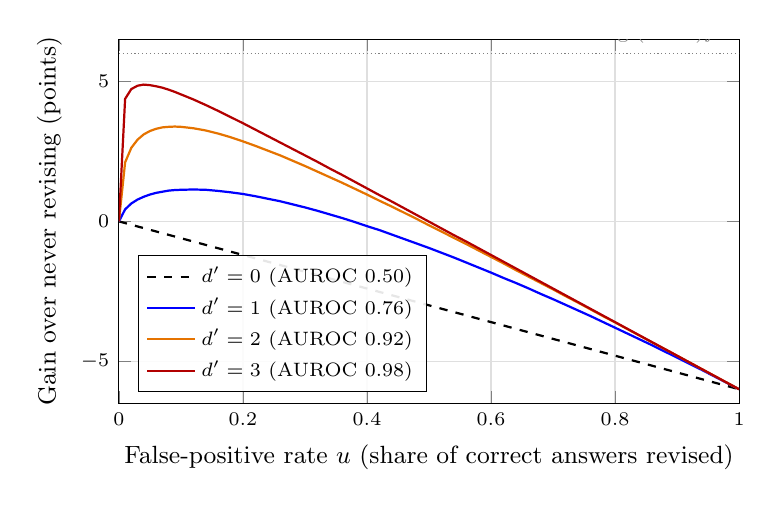
\begin{tikzpicture}
\begin{axis}[
  width=0.78\linewidth, height=6.2cm,
  xlabel={False-positive rate $u$ (share of correct answers revised)},
  ylabel={Gain over never revising (points)},
  xmin=0, xmax=1, ymin=-6.5, ymax=6.5,
  grid=major, grid style={gray!25},
  legend pos=south west, legend style={font=\scriptsize, fill=white, fill opacity=0.9, text opacity=1},
  tick label style={font=\scriptsize}, label style={font=\small},
]
\addplot[thick, dashed, black] coordinates {(0,0) (1,-6)};
\addlegendentry{$d'=0$ (AUROC 0.50)}
\addplot[thick, blue] coordinates {(0.000,0.00) (0.010,0.43) (0.020,0.64) (0.030,0.78) (0.040,0.88) (0.050,0.96) (0.060,1.02) (0.070,1.06) (0.080,1.10) (0.090,1.12) (0.100,1.13) (0.120,1.14) (0.140,1.13) (0.160,1.09) (0.180,1.04) (0.200,0.98) (0.220,0.90) (0.240,0.81) (0.260,0.72) (0.280,0.61) (0.300,0.50) (0.320,0.38) (0.340,0.25) (0.360,0.12) (0.380,-0.02) (0.400,-0.17) (0.420,-0.31) (0.440,-0.47) (0.460,-0.63) (0.480,-0.79) (0.500,-0.95) (0.520,-1.12) (0.540,-1.29) (0.560,-1.47) (0.580,-1.65) (0.600,-1.83) (0.620,-2.02) (0.640,-2.20) (0.660,-2.39) (0.680,-2.59) (0.700,-2.78) (0.720,-2.98) (0.740,-3.18) (0.760,-3.38) (0.780,-3.59) (0.800,-3.80) (0.820,-4.01) (0.840,-4.22) (0.860,-4.43) (0.880,-4.65) (0.900,-4.87) (0.920,-5.09) (0.940,-5.31) (0.960,-5.54) (0.980,-5.77) (1.000,-6.00)};
\addlegendentry{$d'=1$ (AUROC 0.76)}
\addplot[thick, orange!90!black] coordinates {(0.000,0.00) (0.010,2.11) (0.020,2.63) (0.030,2.92) (0.040,3.11) (0.050,3.23) (0.060,3.31) (0.070,3.36) (0.080,3.38) (0.090,3.39) (0.100,3.38) (0.120,3.33) (0.140,3.25) (0.160,3.14) (0.180,3.01) (0.200,2.86) (0.220,2.70) (0.240,2.53) (0.260,2.36) (0.280,2.17) (0.300,1.98) (0.320,1.78) (0.340,1.58) (0.360,1.38) (0.380,1.17) (0.400,0.96) (0.420,0.74) (0.440,0.53) (0.460,0.31) (0.480,0.09) (0.500,-0.14) (0.520,-0.36) (0.540,-0.59) (0.560,-0.81) (0.580,-1.04) (0.600,-1.27) (0.620,-1.50) (0.640,-1.74) (0.660,-1.97) (0.680,-2.20) (0.700,-2.43) (0.720,-2.67) (0.740,-2.90) (0.760,-3.14) (0.780,-3.38) (0.800,-3.61) (0.820,-3.85) (0.840,-4.09) (0.860,-4.33) (0.880,-4.56) (0.900,-4.80) (0.920,-5.04) (0.940,-5.28) (0.960,-5.52) (0.980,-5.76) (1.000,-6.00)};
\addlegendentry{$d'=2$ (AUROC 0.92)}
\addplot[thick, red!70!black] coordinates {(0.000,0.00) (0.010,4.38) (0.020,4.73) (0.030,4.85) (0.040,4.89) (0.050,4.87) (0.060,4.83) (0.070,4.78) (0.080,4.71) (0.090,4.63) (0.100,4.54) (0.120,4.36) (0.140,4.16) (0.160,3.95) (0.180,3.73) (0.200,3.51) (0.220,3.28) (0.240,3.05) (0.260,2.82) (0.280,2.59) (0.300,2.36) (0.320,2.13) (0.340,1.89) (0.360,1.66) (0.380,1.42) (0.400,1.18) (0.420,0.94) (0.440,0.71) (0.460,0.47) (0.480,0.23) (0.500,-0.01) (0.520,-0.25) (0.540,-0.49) (0.560,-0.72) (0.580,-0.96) (0.600,-1.20) (0.620,-1.44) (0.640,-1.68) (0.660,-1.92) (0.680,-2.16) (0.700,-2.40) (0.720,-2.64) (0.740,-2.88) (0.760,-3.12) (0.780,-3.36) (0.800,-3.60) (0.820,-3.84) (0.840,-4.08) (0.860,-4.32) (0.880,-4.56) (0.900,-4.80) (0.920,-5.04) (0.940,-5.28) (0.960,-5.52) (0.980,-5.76) (1.000,-6.00)};
\addlegendentry{$d'=3$ (AUROC 0.98)}
\addplot[thin, gray, densely dotted] coordinates {(0,6) (1,6)};
\node[font=\scriptsize, gray, anchor=south east] at (axis cs:0.98,6) {oracle ceiling $(1-a)f$};
\end{axis}
\end{tikzpicture}
\caption{Gain of confidence gating over never revising, as a function of the share of correct answers that are revised, computed from Eq.~\eqref{eq:gated} with hypothetical parameters $a=0.80$, $b=0.15$, $f=0.30$ and binormal ROC curves of separation $d'$. The right end ($u=1$) corresponds to always revising ($-6$ points). The figure illustrates the model only; it does not show experimental data.}
\label{fig:theory}
\end{figure}
